%%%%%%%%%%%%%%%%%%%%%%%%%%%%%%%%%%%%%%%%%%%%%%%%%%%%%%%%%%%%%%%%%%%%%%%%%%%%%
%%%
%%% File: thesis.tex, version 0.2, May 2020
%%%
%%% =============================================
%%% This file contains a template that can be used with the package
%%% cs.sty and LaTeX2e to produce a thesis that meets the requirements
%%% of the Computer Science Department from the Technical University of Cluj-Napoca
%%%%%%%%%%%%%%%%%%%%%%%%%%%%%%%%%%%%%%%%%%%%%%%%%%%%%%%%%%%%%%%%%%%%%%%%%%%%%

\documentclass[12pt,a4paper,twoside]{report}
\usepackage{textcomp}
\usepackage{cs}
\usepackage{times}
\usepackage{graphicx}
\usepackage{latexsym}
\usepackage{amsmath,amsbsy}
\usepackage{amssymb}
\usepackage[matrix,arrow]{xy}
\usepackage{ae,aecompl}
\usepackage{amstext}
\usepackage{graphics}
\usepackage{ae,aecompl}
\usepackage{algorithm}
\usepackage{algorithmic}
\usepackage{color}
\usepackage{listings}

\usepackage{tabularx}

\usepackage{hyperref}

\usepackage[english,romanian]{babel}
\usepackage{pgfpages}

\usepackage{ucs}
\usepackage[utf8]{inputenc}
\usepackage[T1]{fontenc}



\lstset{%
    language=C,
    basicstyle=\ttfamily,
    keywordstyle=\bfseries,
    commentstyle=\itshape,
    escapechar=\#,
    emphstyle=\bfseries\color{red}
 }


\usepackage{ifpdf}

\graphicspath{{figures/}}
\ifpdf
  \DeclareGraphicsExtensions{.pdf,.jpeg,.png}
\else
  \DeclareGraphicsExtensions{.eps}
\fi

% \mastersthesis
\diplomathesis
% \leftchapter
\centerchapter
% \rightchapter
\singlespace
% \oneandhalfspace
% \doublespace

\renewcommand{\thesisauthor}{Prenume NUME}    %% Your name.
\renewcommand{\thesismonth}{Septembrie}     %% Your month of graduation.
\renewcommand{\thesisyear}{2025}      %% Your year of graduation.
\renewcommand{\thesistitle}{TITLUL LUCRĂRII DE DISERTAȚIE}
\renewcommand{\thesissupervisor}{titlul științific Prenume NUME}
\newcommand{\utcnlogo}{
\includegraphics[width=14.5cm]{sigla.jpg}}

%\renewcommand{\thesisdedication}{P'arin'tilor mei}

\begin{document}

\begin{titlepage}
\vspace*{-3cm}
%\noindent \includegraphics*[width=6.04in, height=0.98in, keepaspectratio=false]{sigla}
\utcnlogo
\begin{center}
\textbf{FACULTATEA DE AUTOMATICĂ ȘI CALCULATOARE}\\
\textbf{DEPARTAMENTUL CALCULATOARE}\\

\vspace{5cm}

\Large {\textbf\thesistitle \\}
\vspace {1cm}
\large {LUCRARE DE DISERTAȚIE}\\

\vspace{8cm}

%\newcolumntype{R}{>{\raggedleft\arraybackslash}X}%
\begin{tabularx}{\textwidth}{r l}  
Absolvent masterand:   &  \textbf\thesisauthor \\
 & \\
Coordonator științific:  & \textbf\thesissupervisor \\
\end{tabularx}

\vspace{2.5cm}

%\vspace{\stretch{1}}
\thesismonth, \thesisyear %Iulie, 2025\\
\end{center}
\end{titlepage}

\begin{titlepage}
\phantom{1}
\end{titlepage}


\begin{titlepage}
\vspace*{-3cm}
%\noindent \includegraphics*[width=6.04in, height=0.98in, keepaspectratio=false]{sigla}
\utcnlogo
\begin{center}
\textbf{FACULTATEA DE AUTOMATICĂ ȘI CALCULATOARE}\\
\textbf{DEPARTAMENTUL CALCULATOARE}\\

\vspace{1cm}

\newcolumntype{R}{>{\raggedleft\arraybackslash}X}%
\begin{tabularx}{\textwidth}{lR}
DECAN & DIRECTOR DEPARTAMENT \\
\textbf{Prof.Dr.Ing. Vlad MUREȘAN} & \textbf{Prof.Dr.Ing. Rodica POTOLEA}\\
\end{tabularx}

\vspace {3.5cm}

Student masterand:  \textbf\thesisauthor
\vspace{1cm}

\large \textbf\thesistitle \\
\vspace {1cm}

\end{center}

% \vspace{1cm}

\begin{flushleft}
\begin{enumerate}
 \item \textbf{Enunțul temei:} \textit{Scurtă descriere a temei lucrării de disertație și datele inițiale}

 \item \textbf{Conținutul lucrării:} \textit{(enumerarea părților componente) Exemplu: Pagina de prezentare, aprecierile coordonatorului, titlul capitolului 1, titlul capitolului 2, \dots, titlul capitolului n, bibliografie, anexe.}

 \item \textbf{Locul documentării:} \textit{Exemplu:} UTCN, Cluj-Napoca

 \item \textbf{Consultanți:} 

 \item \textbf{Data emiterii temei:} \textit{Exemplu:} 1 noiembrie 2024

 \item \textbf{Data predării:} \textit{Exemplu:} 8 septembrie 2025
\end{enumerate}

\end{flushleft}

\vspace{3.5cm}

\begin{center}
\newcolumntype{R}{>{\raggedleft\arraybackslash}X}%
\begin{tabularx}{\textwidth}{X X}  %{lR}
 & Student masterand: \dotfill \\
 & \\
 & Coordonator științific: \dotfill \\
\end{tabularx}

%\vspace{\stretch{1}}


\end{center}

\end{titlepage}


\begin{titlepage}
\phantom{1}
\end{titlepage}


\begin{titlepage}
\vspace*{-3cm}
%\noindent \includegraphics*[width=6.04in, height=0.98in, keepaspectratio=false]{sigla}
\utcnlogo
\begin{center}
\textbf{FACULTATEA DE AUTOMATICĂ ȘI CALCULATOARE}\\
\textbf{DEPARTAMENTUL CALCULATOARE}\\
\end{center}

\vspace{2cm}

\begin{center}
\textbf{Declarație pe proprie răspundere privind \\
autenticitatea lucrării de disertație}
\end{center}

\vspace{1cm}

Subsemnatul(a) \thesisauthor, legitimat(ă) cu \dots \dots seria \dots \dots nr. \dots \dots \dots, 
CNP \dots \dots \dots \dots \dots \dots \dots \dots, autorul lucrării \thesistitle, elaborată  în vederea susținerii
examenului de finalizare a studiilor de disertație la Facultatea de Automatică și Calculatoare, specializarea 
\dots \dots \dots \dots \dots \dots \dots \dots \dots \dots \dots \dots \dots, din cadrul Universității 
Tehnice din Cluj-Napoca, sesiunea \dots \dots \dots \dots a anului universitar 2024-2025, declar pe
proprie răspundere că această lucrare este rezultatul propriei activități intelectuale, pe baza cercetărilor mele
şi pe baza informațiilor obținute din surse care au fost citate în textul lucrării și în bibliografie.

Declar că această lucrare nu conține porțiuni plagiate, iar sursele bibliografice au fost folosite cu respectarea
legislației române și a convențiilor internaționale privind drepturile de autor.

Declar, de asemenea, că această lucrare nu a mai fost prezentată în fața unei alte comisii de examen de disertație.

În cazul constatării ulterioare a unor declarații false, voi suporta sancțiunile administrative, respectiv,
\textit{anularea examenului de disertație}.

Sunt de acord ca, pe tot parcursul vieții, în cazul în care este necesar și se va dori verificarea
autenticității lucrării mele să fiu identificat și verificat în baza datelor declarate de mine.
\vspace{3cm}

\newcolumntype{R}{>{\raggedleft\arraybackslash}X}%
\hspace{-1cm}\begin{tabularx}{\textwidth}{l R l}  %{lR}
Data & \thesisauthor & \\
& \\
\dots \dots \dots \dots  &  \dots \dots \dots \dots \dots \dots \dots \dots &  \\
& \textit{Semnătura} &
\end{tabularx}


\end{titlepage}


\begin{titlepage}
\phantom{1}
\end{titlepage}


%\pagestyle{headings}

\newenvironment{definition}[1][Definiție.]{\begin{trivlist}
\item[\hskip \labelsep {\bfseries #1}]}{\end{trivlist}}

% ABSTRACT
%\begin{abstract}
% Descrierea sumară a lucrării, în câteva fraze.
%\end{abstract}

%\begin{titlepage}
%\phantom{1}
%\end{titlepage}

%\thesistitle                    %% Generate the title page.
%\authordeclarationpage                %% Generate the declaration page.

\pagenumbering{roman}
\setcounter{page}{1}

\tableofcontents
\newpage

%\listoftables
%\listoffigures

\clearpage
\newpage

\pagenumbering{arabic}
\setcounter{page}{1}


%\setcounter{page}{\value{page}}
\chapter{Introducere}
\label{cap:Introducere}
%\setcounter{page}{7}
%\addtocounter{page}{6}
\pagestyle{headings}
Ce se scrie aici:
\begin{itemize}
    \item Contextul
    \item Conturarea domeniului exact al temei
    \item Se răspunde la întrebările: \textbf{ce} (s-a făcut)?, \textbf{de ce} (s-a făcut, adică motivația; ce se rezolvă, la ce este util, etc.)?, \textbf{cum} (s-a făcut, adică particularitățile abordării, prezentate sumar).
    \item Introducerea se termină cu o descriere a conținutului lucrării, de genul: Cap X descrie ..., Cap Y prezintă ...
    \item Introducerea reprezintă o sinteză a lucrării, din care cititorul trebuie să-și poată da bine seama dacă lucrarea prezintă sau nu interes pentru el. 
\item reprezintă cca 5\% din lucrare
\end{itemize}

\section{Contextul proiectului}
Subcapitolul este scris cu font Times New Roman 14 puncte, bold. Pentru numerotare se folosesc cifre arabe, de ex: $X.Y$ unde X reprezintă numărul capitolului, iar Y numărul subcapitolului. Distanța de la titlul subcapitolului până la primul rând scris este de 8 puncte.

\subsection{Subsecțiune}
Distanța înainte și după titlul subcapitolului este de 8 puncte (acest lucru este realizat implicit în fișierul de stil furnizat). 
Fiecare tabel introdus în lucrare este numerotat astfel: Tabel $x.y$ unde x reprezintă numărul capitolului, iar y numărul tabelului din capitol. 
Se lasă o distanță de 8 puncte între text și tabel. (tabelul \ref{table:nonlin}).
\begin{table}[ht]
\centering                          % tabel centrat 
\begin{tabular}{|c|c|c|c|}          % 4 coloane centrate 
\hline\hline                        % linie orizontala dubla
Case & Method\#1 & Method\#2 & Method\#3 \\ [0.5ex]   % inserare tabel
%heading
\hline                              % linie orizontal simpla
1 & 50 & 837 & 970 \\               % corpul tabelului 
2 & 47 & 877 & 230 \\
3 & 31 & 25 & 415 \\[1ex]           % [1ex] adds vertical space
\hline                              
\end{tabular}
\caption{Nonlinear Model Results}   % titlul tabelului
\label{table:nonlin}                % \label{table:nonlin} introduce eticheta folosita pentru referirea tabelului in text; referirea in text se va face cu \ref{table:nonlin}
\end{table}

Fiecare figură introdusă în text este citată (de ex: în figura $x.y$ este prezentată ...) și numerotată.
Numerotarea se face automat astfel: Figura $x.y$ unde x reprezintă numărul capitolului, iar y numărul figurii din acel capitol. Ex: figura \ref{fig:imag}

\begin{figure}[h]
    \centering
    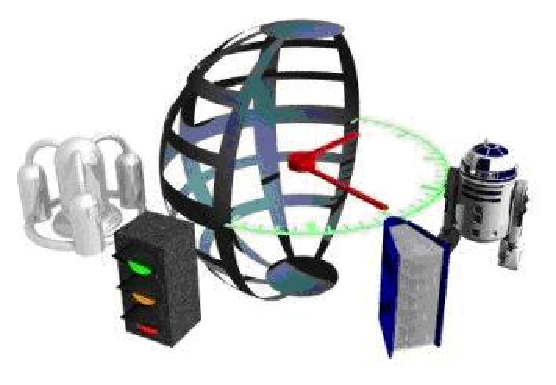
\includegraphics[]{image}	%numele fisierului
    \caption{Numele figurii}
    \label{fig:imag}
\end{figure}


Ecuații:
\begin{equation}
    \Delta =\sum_{i=1}^N w_i (x_i - \bar{x})^2 .
\end{equation}

\subsection{Alte exemple în \LaTeX}
\label{subsec:s10} %aceasta trebuie adaugat pentru a referi o sectiune  

Modus ponens modificat: 
% aceasta este o ecuatie 
\begin{equation} 
  \frac{a \land a \rightarrow b}
       {b}
\label{eq:e50}
\end{equation}

Acolada: 

\[\left \{ 
    \begin{array}{l}
        p =\frac{x}{x+y+z} \\
        q = \frac{y}{x+y+z}\\ 
        r = \frac{z}{x+y+z}
    \end{array}\right.
\]
        
Itemi ne-numerotați:  
\begin{itemize}
    \item numărul 1 
    \item numărul 2 
    \item numărul 3 
\end{itemize}

Itemi numerotați:
\begin{enumerate}
    \item numărul 1 
    \item numărul 2 
    \item numărul 3 
\end{enumerate}

%asa se citeaza o lucrare                    
Anumiți autori spun că  \cite{Zhou04} 


Un tabel mai complicat este \ref{Mom}.
\begin{table}
      \begin{center}
            \begin{tabular}{|l|l|l|l|l|l|l|}
                \hline 
                & \multicolumn{3}{c|}{belief} & \multicolumn{3}{c|}{atomicity} \\
                \cline{2-7}
                & $poor$ & $avg$ & $good$ & $poor$ & $avg$ & $good$ \\ 
        	\hline
                $success$   &  0.1    &  0.2    &  0.3    & 0.4    & 0.5    &  0.6     \\
                $failure$   &  0.1    &  0.2    &  0.3    & 0.4    & 0.5    &  0.6     \\
                                                    \hline
	    \end{tabular}
        \end{center}
    \caption{Multiplicarea Opiniilor Multinomiale}
    \label{Mom}
\end{table}

                                                                                                                                                                                                                                                                  
Un algoritm poate fi scris astfel:
%\usepackage{algorithm} si \usepackage{algorithmic}  trebuie incluse la inceputul documentului

\begin{algorithm}
 \caption{Commitment decision}
  \label{ftalg}
   \begin{algorithmic}
     \IF{$Committed(G_{1},GR,\alpha)$} 
      \STATE $BRT_{\alpha}$ = $PredictBRT(G_{1},GR,\alpha,C_{GR})$
      \STATE $C_{\beta}$ = $ContextUpdate(C_{\beta},o)$
      \STATE $BRT_{\beta}$ = $PredictBRT(G_{1},G_{2},\beta,C_{\beta})$
      \STATE $BRT_{\alpha}^{o}$ = $BRTReplace(BRT_{\alpha},BRT_{\beta})$
      \STATE $utility$ = $Eval(BRT_{\alpha}^{o})-Eval(BRT_{\alpha})$
     \ENDIF
      \IF{$utility \ge CommunicationCost(G_{2})$}
        \STATE $Int.To(G_{1},Communicate(G_{1},G_{2},o))$
      \ENDIF
   \end{algorithmic}
\end{algorithm}

\section*{Mulțumiri}
Mulțumiri lui Aristotel pentru Secțiunea \ref{subsec:s10} %Asa se refera o sectiune

\include{ch2}
\chapter{Studiu bibliografic/Stadiul actual în domeniu}

Documentarea bibliografică are ca obiectiv prezentarea stadiului actual al domeniului/ sub-domeniului în care se situează tema, prezentarea cercetărilor similare şi raportarea abordării din lucrare la acestea. 

Acest capitol reprezintă cca. 10--15\% din lucrare.

Referințele se scriu în secțiunea Bibliografie. Formatul referințelor trebuie să fie de tipul IEEE sau asemănător. 

Referințele bibliografice se vor face pentru fiecare carte, articol sau material folosit pentru elaborarea lucrării de disertație. 

În secțiunea Bibliografie sunt exemple de referințe pentru articol la conferințe sau seminarii  \cite{Zhou04}, articol în jurnal \cite{Antoniou04}, sau cărți \cite{strunk}. 

Referințele spre aplicații sau resurse online (pagini de internet) trebuie să includă cel puțin o denumire sugestivă pe lângă link-ul propriu zis \cite{webpage}, plus alte informații dacă sunt disponibile (autori, an, etc.). Referințele care prezintă doar link spre resursa online se vor plasa în footer-ul paginii unde sunt referite.

Citarea referințelor în text este obligatorie, vezi exemplul de mai jos (în funcție de tema proiectului se poate varia modul de prezentare a metodei/aplicației).

\section{Abordări similare}

Citarea referințelor se face ca în exemplele din \ref{subsec:s10}, de mai sus și din citările următoare.

În articolul \cite{Antoniou04} autorul descrie configurația tehnică a unei "honeynet" și prezintă câteva atacuri de actualitate asupra honeynet, precum și o serie de recomandări pentru securizarea sistemelor conectate la rețele de calculatoare.

În capitolul 4 al \cite{strunk}, \dots.








\chapter{Prezentarea proiectului}

\section{Precizări asupra conținutului și a modului de organizare}

Împreună cu capitolul următor reprezintă cca. 70\% din lucrare. 

Titlul acestui capitol nu este unul impus și nici nu corespunde neapărat unui singur capitol. 
Titlul indică mai degrabă o parte (importantă și centrală, de altfel) a lucrării, în care se prezintă 
ceea ce s-a realizat efectiv: contribuțiile autorului. Organizarea acestei părți este dependentă și 
specifică fiecărei lucrări în parte și este stabilită de către fiecare autor după cum i se pare mai 
potrivit pentru tema lui. Ea poate cuprinde prezentarea unor concepte teoretice (unelte sau tehnici
matematice folosite în lucrare, prezentarea sau introducerea unor concepte teoretice etc.),  o 
analiză a diferitelor metode/algoritmi/tehnologii etc. luate în considerare sau dezvoltate de către 
autor, o prezentare a unui design (mai mult sau mai puțin detaliat) sau chiar detalii a unei 
eventuale implementări/prototip, dacă e cazul.

Trebuie remarcat însă faptul că această parte reprezintă contribuția personală a autorului, și în nici 
un caz ea nu poate fi sinteza unor texte preluate din alte surse. Prin urmare, orice informații sunt 
prezentate aici, ele trebuie să corespundă cel puțin unei interpretări/analize critice personale a 
autorului, dacă nu chiar unor idei originale ale acestuia. 


\subsection{Subsecțiune}


\include{ch5}
\chapter{Concluzii}


\section{Conținut}

\begin{itemize}
 \item un rezumat al contribuțiilor aduse
 \item a analiză critică a rezultatelor obținute: avantaje, dezavantaje, limitări
 \item o descriere a posibilelor dezvoltări și îmbunătățiri ulterioare
\end{itemize}


\section{Detalii tehnice}

\subsection{Dimensiune}

Cca 3--5\% din total.








% \include{ch7}
% \include{ch8}

%\addcontentsline {toc}{chapter}{Bibliography}
\bibliographystyle{IEEEtran}
\bibliography{thesis}%same file name as for .bib

\include{apendix}

\end{document}
